\documentclass[a4paper,10pt]{article}
\usepackage{amsmath}
\usepackage{amsthm}
\newtheorem{mydef}{Definition}
\usepackage{url, hyperref}
\usepackage{amsthm}
\usepackage{amsfonts}
\usepackage{amssymb}
\newtheorem{theorem}{Theorem}
\newtheorem{lemma}{Lemma}
\usepackage{fullpage}
\usepackage{tikz}
\usepackage{float}
\usepackage{listings}
\usepackage{color}
\definecolor{dkgreen}{rgb}{0,0.6,0}
\lstset{language=Matlab,
   keywords={break,case,catch,continue,else,elseif,end,for,function,
      global,if,otherwise,persistent,return,switch,try,while},
   basicstyle=\ttfamily,
   keywordstyle=\color{blue},
   commentstyle=\color{dkgreen},
   stringstyle=\color{magenta},
   numbers=left,
   numberstyle=\tiny\color{gray},
   stepnumber=1,
   numbersep=10pt,
   backgroundcolor=\color{white},
   tabsize=4,
   showspaces=false,
   showstringspaces=false}
\usepackage{mathtools}
\usepackage[T1]{fontenc}
\usepackage{subfigure}
\usepackage{algorithm}
\usepackage{algpseudocode}
\bibliographystyle{plain}

\title{Project Proposal: Efficient segmentation algorithms for shark fin
identification}
\author{L. Cilli\'{e}, 16010450}
\date{August 1, 2013}

\begin{document}
\maketitle
\lstset{language=Matlab}

\newpage
\tableofcontents
\newpage

\section{Problem statement and motivation}  
Just as humans are identified by their fingerprints, sharks have an unique
dorsal fin structure.  Identifying shark sightings these days can be very
valuable.  In order to do that and also to match shark sightings, photos of
shark fins, as will be shown in the proposal, will be analysed by a computer. 
This will consist of comparing the edges in the image and segmenting the
foreground, the shark fin being most prominent,  from the background, the sea. 
Although the photos provided are of a good quality and only include the fin, the
foreground and background properties can still vary significantly, making this a
non-trivial problem.  This project aims to investigate efficient segmentation
algorithms for shark fin identification.  The approach will consist of
evaluating (by means of a computer) different methods for classifying foreground
and background, as well as segmenting the foreground successfully.  By doing so,
the burden on biological researchers can be reduced. 

\begin{figure}[H]
\centering
\mbox{\subfigure[Shark fin 1]{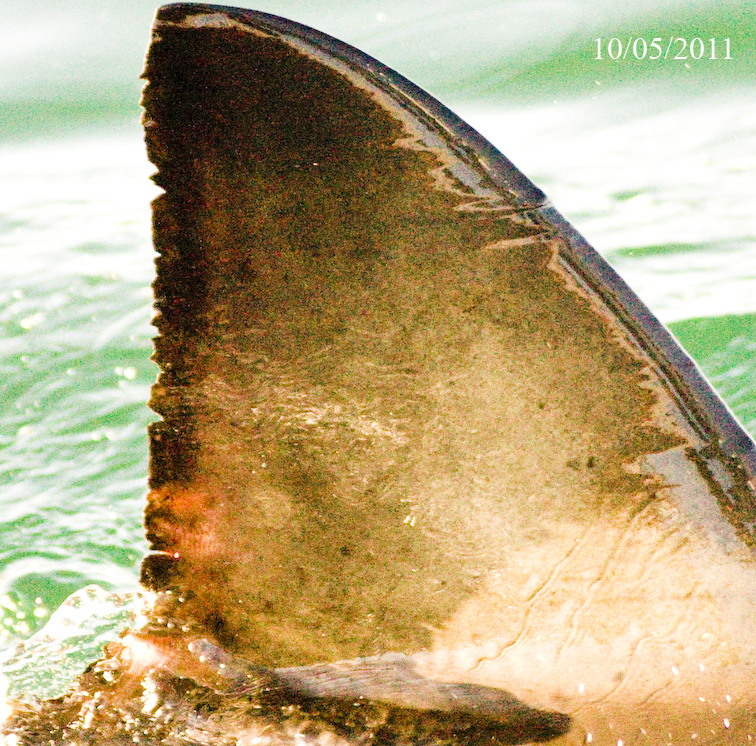
\includegraphics[width=1in]{haai1.jpg}} \quad
\subfigure[Shark fin 2]{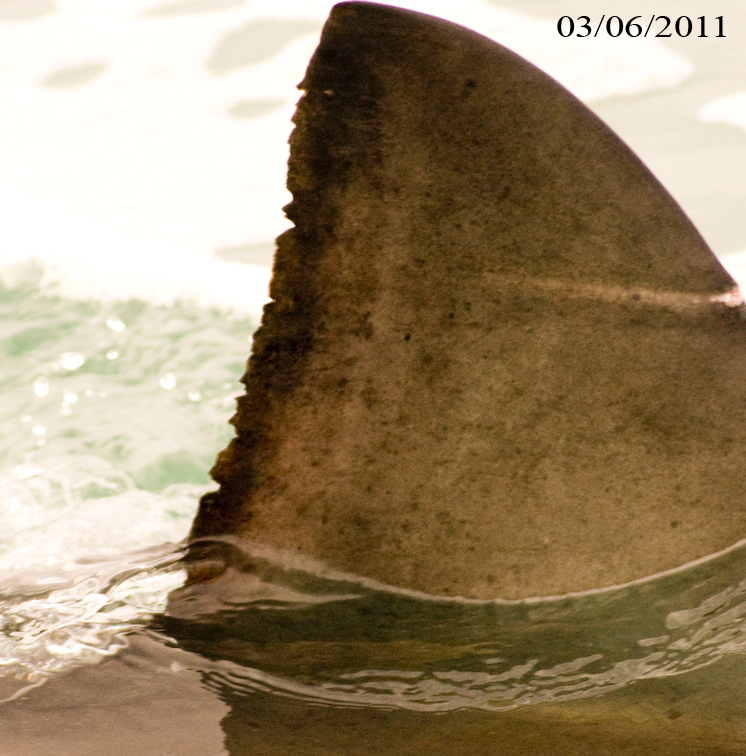
\includegraphics[width=1in]{haai2.jpg}}}
\caption{Examples of shark fin images}
\end{figure}

\section{Background}
Image segmentation is well known in the field of image processing.  It consists
of partitioning a digital image into multiple segments for some or other reason.
 Usually to make the image easier to analyse.  In other words each pixel is
assigned a label and all the pixels with the same label share a certain
property.  Image segmentation is typically used to locate an object or
boundaries in an image.  Well known examples where image processing are used is
in medical imaging to locate tumours for example, face and
fingerprint recognition and video surveillance.


\section{Segmentation algorithms}
\subsection{Different categories and techniques}
Segmentation algorithms can be arranged into different categories \cite{is}. 
Some of the most well-known categories are
\begin{itemize}
 \item \textbf{Thresholding} \cite{is} Possibly the most basic method in the
field.  It relies on selecting the best threshold value to convert a gray-scale
image into a binary image.  Segmentation is then done on the binary image. 
 \item \textbf{Clustering} \cite{is} For these methods, the $K$-means algorithm
is typically used to partition an image into $K$ clusters, whereafter
segmentation will follow.
 \item \textbf{Compression-based} \cite{is} This method conjectures that the
optimal segmentation is the one that minimizes, when considering all possible
segmentations, the coding length of the data.
 \item \textbf{Histogram-based} \cite{is} This is a very efficient method in the
sense that it only passes through all the pixels once.  Then a histogram of all
the pixels in the image is computed.  The peaks and valleys, colour intensity
can be used as a measure, are then used to locate clusters in the image.
 \item \textbf{Edge detection} \cite{is} Edge detection is a well-developed
field in image processing.  Region boundaries and edges are closely related,
since there are usually a sharp adjustment at region boundaries.  Edge detection
techniques can therefore be used as a bases for different segmentation
algorithms.  
 \item \textbf{Region growing} \cite{is}  This method takes as input not only
the image, but also a set of seeds, which marks the objects to be segmented. 
Thereafter neighbouring, unallocated pixels are compared to the specific seed
point.  That is how the region grows iteratively.  The pixels are compared using
the difference between intensity value and the region's mean.  Pixels are then
allocated to a specific region if that difference is a minimum.  The process
terminates if all pixels belong to a region.  
 \item \textbf{Watershed transformation} \cite{is} See description in 3.2.    
 \item \textbf{Graph partitioning} \cite{is} This method is based on modelling
the image as a weighted, undirected graph, where the nodes represent the pixels
and the weights represent the similarity between neighbouring pixels. Then the
graph is partitioned into clusters according to a specific criterion.  Each
partition is then considered an object segment in the image.       
 \item \textbf{Trainable} \cite{is} Also known as Neural network segmentation,
this process involves processing the small areas of an image by means of an
artificial neural network or a set of neural networks.  Thereafter, using the
categories recognised by the network, the decision-making mechanism marks the
image accordingly and segmentation is done.
\end{itemize}

\subsection{The Watershed algorithm}
One of the first algorithms tested was the classic watershed algorithm, as
implemented in \cite{scikit}.  The algorithm starts with user-defined markers,
called seed points, which can be viewed as little holes in the image, whereafter
pixel values are treated as a topography/landscape.  The algorithm then floods
basins from the user-defined markers until basins which attribute to different
markers meet at watershed lines.  In this case marker positions are chosen as
the local maxima of the image.  Thereafter the segmentation is done on the
gradient image.  The result of the watershed algorithm applied to a shark fin
image is shown below.

\begin{figure}[H]
\centering
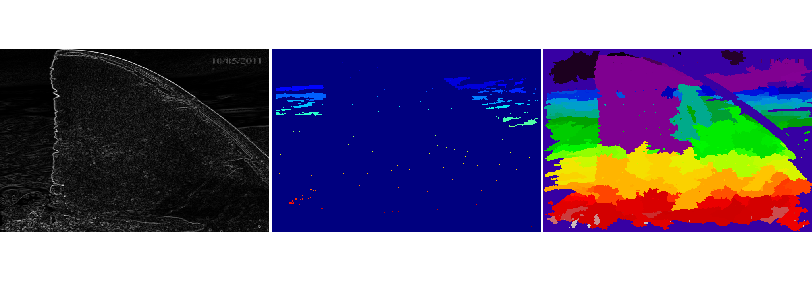
\includegraphics[width=4in,height=2in]{watershed.png} 
\label{fig1}
\caption{Result using the watershed algorithm}
\end{figure}

\noindent The first image shows the gradient image of the original shark fin
image.  The second image shows the pixels that are identified as a local maxima.
 The third image shows how the basins flooded until watershed lines are reached.
 Putting the correct segments together, which will require a lot of hard work,
an effective segmentation can be done.

\subsection{The Random Walker algorithm}
The basic method (from the graph partitioning category shown above), as
described in \cite{rw} and \cite{rw1}, is as follows.  The user labels a few
pixels as foreground or background for example.  This is then called the seeds. 
A random walker is then released from each of the unlabelled pixels. 
Thereafter, the probability that a certain pixel's random walker first arrives
at a seed with a label, is computed.  In other words, if the user labels $n$
pixels, each with a different label, then the probability that the random walker
leaving the pixel will first arrive at a certain labelled pixel, must be
computed.  The latter is done by modelling the image as a weighted graph, where
the weight of an edge reflects the similarity(intensity values) between pixels,
and solving a system of linear equations.  The pixel is then assigned the label
of the seed for which it is most likely to reach.  The process is repeated until
each pixel is assigned a specific label. 

\subsection{Random forests as a semantic segmentation algorithm}
A semantic segmentation algorithm is done by assigning category labels to a set
of super pixels obtained by clustering the joint colour space and coordinate
space using the mean shift algorithm \cite{ms}.
The method of interactive semantic segmentation as in \cite{RF} can be described
as follows.  Each image is presented as a set of super pixels, where a super
pixel is a set of neighbouring pixels.  The first image in the data set can be
segmented with any appropriate segmentation algorithm.  An appearance model is
created.  The next image is now segmented automatically using the appearance
model. \\  

\noindent During the segmentation the user may correct mistakes by relabelling
and thus updating the appearance model.  Every time the user approves the
segmentation, the system learns from the new labelling information. As image
segmentation continues, user time spent on correcting labels reduces and thus
the rate of image labelling increases.  \\

\noindent This method can be helpful in the sense that it works with a database
of images of the same kind.  Since the shark fin images are all of the same
type, it would be very beneficial to manually segment the first image only and
then automatic segmentation will follow.  By updating the appearance model, one
can also be certain that better segmentation results will follow.  \\  

\section{The region growing GrowCut algorithm}
\subsection{What is a cellular automaton?}
A cellular automaton consists of a grid of cells, where each one of the cells
can be in a finite number of states, say on and off.  This must be specified
beforehand.  Around each cell, a set of cells, called the cell's neighbourhood,
is defined.  An initial state, at time t = 0, is also assigned to each cell.  A
new generation of cells is then created according to a fixed rule or
mathematical function that determines the new state of the cell, by looking at
the current state of the cell as well as that of its neighbourhood.  This rule
is then applied to all of the cells simultaneously.  In this way, the cell's
state gets updated.  Note that the rules for each cell are the same and do not
change over time.  Two of the most common neighbourhood systems used are the Von
Neumann neighbourhood and the Moore neighbourhood which are shown below. 
Probably the most well-known example of a two dimensional automaton is Conway's
Game of Life.  See \cite{gol} for further details.

\begin{figure}[H]
\centering
\mbox{\subfigure{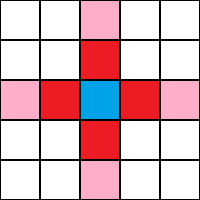
\includegraphics[width=1in]{VonNeumann.png}} \quad
\subfigure{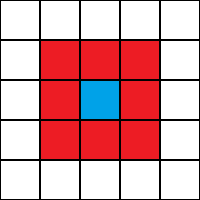
\includegraphics[width=1in]{Moore.png}}} \caption{Von Neumann and
Moore neighbourhood systems \cite{n}}
\end{figure}

\subsection{The GrowCut algorithm as implemented in Python}
The GrowCut algorithm \cite{alg} is an interactive, multi-label segmentation
algorithm for N-dimensional images.  The algorithm is based on cellular
automata, i.e.,  the user labels a few pixels and the rest of the image is then
segmented automatically by a cellular automaton. \\

\noindent The pseudo code for the automata evolution rule is shown below. 
\begin{algorithm}[H]
\begin{algorithmic}[1]
 \State // For each cell...
 \For{$\forall p \in P$}
 \State // Copy previous state
 \State $l^{t+1}_{p} = l^{t}_{p}$;
 \State $\theta_{p}^{t+1} = \theta_{p}^{t}$;
 \State // Neighbours try to attack the current cell
 \For{$\forall q \in N(p)$}
 \If{$g(\| \overrightarrow{C}_{p} - \overrightarrow{C}_{q} \|_{2}) \cdot
\theta^{t}_{q} > \theta_{p}^{t}$}
 \State $l^{t+1}_{p} = l^{t}_{q}$
 \State $\theta^{t+1}_{p} = g(\| \overrightarrow{C}_{p} - \overrightarrow{C}_{q}
\|_{2}) \cdot \theta^{t}_{q}$
 \EndIf
 \EndFor
 \EndFor
\end{algorithmic}
\end{algorithm}

\noindent where $g$ is a monotonous decreasing function bounded to $[0, 1]$. 
The function is given by
\[
g(x) = 1 - \frac{x}{max\| \overrightarrow{C} \|_{2}}. 
\]

\noindent The cell state referred to is considered a triplet $(l_{p},
\theta_{p}, \overrightarrow{C}_{p})$, where $l_{p}$ is the label of the cell
($K$ labels in total), $\theta_{p}$ is the 'strength' of the cell and
$\overrightarrow{C}_{p}$ is the cell feature vector.  Without loss of generality
it can be assumed that $\theta_{p} \in [0,1]$. 
The initial state of the pixels is set to $l_{p} = 0, \theta_{p} = 0,
\overrightarrow{C}_{p} = RGB_{p}$, where $RGB_{p}$ is a three dimensional vector
of the pixel's colour in 
the RGB space.  The goal of the segmentation is to assign one of the possible
$K$ labels to each one of the pixels.  The user starts the segmentation by
marking specific pixels as
foreground and others as background.  This sets the initial state of each pixel.
 While the labels are being updated by the rule above, which will be discussed
in greater detail hereafter, the user can correct and guide the process if
desired.  The number of iterations the algorithm has to follow can also be set
beforehand.  \\

\noindent The evolution rule is as follows.  Consider cell $p$.  Now consider
one of the cells in its neighbourhood, type specified beforehand, say cell $q$. 
If the difference in intensity of $p$ and $q$, times the cell strength of $q$,
is greater than the cell strength of $p$, the label of $p$ is updated to the
label of $q$.  Whereas the cell strength of $p$ is updated to the difference in
intensity of $p$ and $q$, times the cell strength of $q$.  These states are then
the starting values for the next iteration. \\

\noindent An interactive implementation of the algorithm, \cite{growcut}, was
received from Dr. Nathan Faggian, Senior Technical Officer at Bureau of
Meteorology, Australia.  The result of his implementation, with changes to the
damping function, applied to one of the shark fin images is shown below. 
\begin{figure}[H]
 \centering
 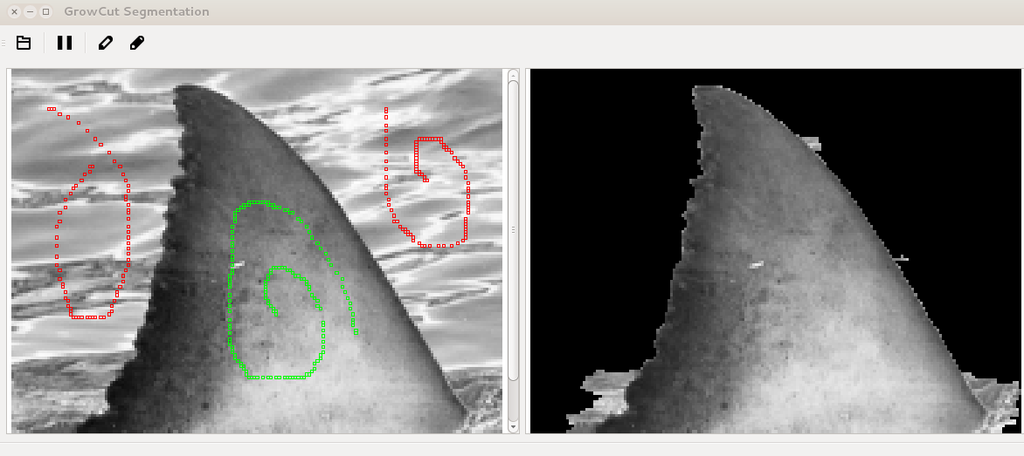
\includegraphics[width=3in, height=1.5in]{haaim}
 \caption{Original Python implementation}
 \label{fin}
\end{figure}    


\noindent Following the pseudo code given above, we developed our own
implementation of the GrowCut algorithm in Python in order to aid our
understanding of the algorithm.  It is now also easier to work on the
optimisation, i.e. speed and quality of the segmentation.  The result of our
own implementation applied to one of the shark fin images, as well as a strength
map of the cells, is shown below
\begin{figure}[H]
 \centering
 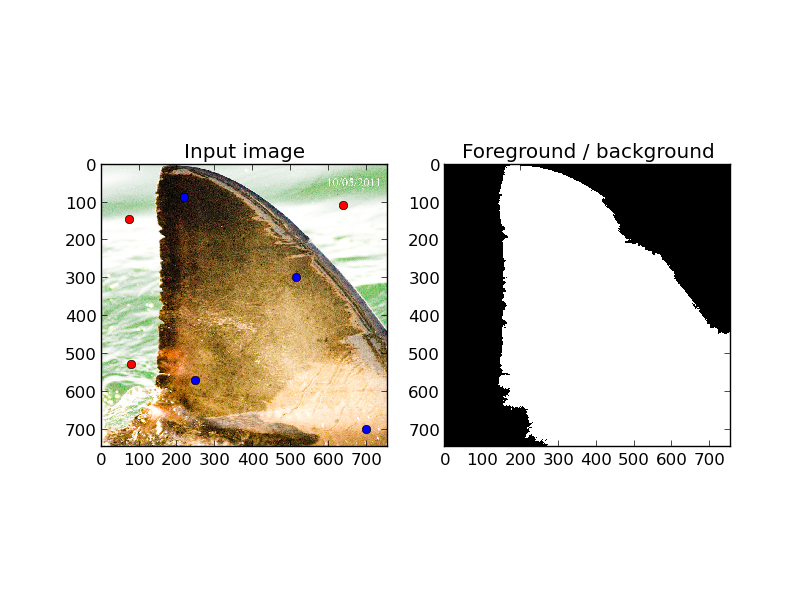
\includegraphics[width=4in, height=1.7in]{demo1.png}
 \caption{Our Python implementation}
\end{figure}   


\noindent Cython \cite{cython} is a language that compiles to a Python extension
module.  It is a super set of the Python language that allows calling
C-functions and declaring C-types on variables and class attributes.  This
results in generating very efficient C-code from Cython code.  Cython was used
to increase the speed of our own basic implementation of the GrowCut algorithm. 
This was one of the steps to better the performance of the segmentation.  \\     

\noindent It is clear that both implementations gave remarkable results and a
definite advantage of this algorithm compared to others, is of course the
simplicity, yet power of each step of the algorithm. 


\section{Objectives}
We aim to achieve the following.
\begin{itemize}
 \item To do an in-depth comparison between the different segmentation
algorithms considered, whereafter sensible conclusions can be made. 
 \item To further study the GrowCut algorithm in order to optimise our
implementation of the algorithm.  To do that, we will look at different
'attacking' strategies, investigate the condition of boundary smoothness and
look at different texture features of the image.
 \item To do a further study on Random Forests as a classification method and
how it can be implemented to be of use.  Also study the topic of conditional
random fields which relates to the latter.
 \item Get the Random Walker segmentation algorithm running on a shark fin
image.
\end{itemize}

\newpage
\bibliography{pp}

\end{document}
